\documentclass[a4paper,12pt]{article}

\usepackage[utf8]{inputenc}

\usepackage{graphicx}

\usepackage{geometry}

\usepackage{caption}

\geometry{margin=1in}
 
\title{Modelo Relacional UML da Aplicação MyRottenPotatoes}

\author{}

\date{}
 
\begin{document}
 
\maketitle
 
\section*{Introdução}

A aplicação \textbf{MyRottenPotatoes} é um sistema desenvolvido em \textit{Ruby on Rails}, frequentemente utilizado para fins educacionais. Essa aplicação permite a gestão de informações relacionadas a filmes, incluindo suas críticas. Este relatório apresenta o modelo relacional UML simplificado para a aplicação, descrevendo suas principais entidades, atributos e relacionamentos.
 
\section*{Entidades Principais}
 
\subsection*{1. Movie (Filme)}

\begin{itemize}

    \item \textbf{id}: Identificador único (chave primária).

    \item \textbf{title}: Título do filme.

    \item \textbf{rating}: Classificação do filme (e.g., PG, G, R).

    \item \textbf{release\_date}: Data de lançamento.

    \item \textbf{description}: Resumo ou sinopse do filme.

\end{itemize}

Relacionamento: Um filme pode ter nenhuma ou várias críticas.
 
\subsection*{2. Review (Crítica/Comentário)}

\begin{itemize}

    \item \textbf{id}: Identificador único (chave primária).

    \item \textbf{movie\_id}: Chave estrangeira associada ao filme.

    \item \textbf{user\_id}: Chave estrangeira associada ao usuário.

    \item \textbf{content}: Conteúdo ou texto da crítica.

    \item \textbf{rating}: Nota atribuída ao filme (e.g., de 1 a 5).

\end{itemize}

Relacionamento: Cada crítica está associada a um filme e a um usuário.
 
 \subsection*{3. User (Usuário)}

\begin{itemize}

    \item \textbf{id}: Identificador único (chave primária).

    \item \textbf{user\_name}: Nome do usuário.

    \item \textbf{password}: Senha criptografada.

    \item \textbf{email}: Email associado ao usuário.

\end{itemize}

Relacionamento: Cada usuário está associado a nenhuma ou várias reviews/crítica.
 
 
\section*{Modelo Relacional UML}
 
Abaixo está o modelo relacional UML que descreve a estrutura de dados da aplicação \textbf{MyRottenPotatoes}:
 
\begin{figure}[h!]

    \centering

    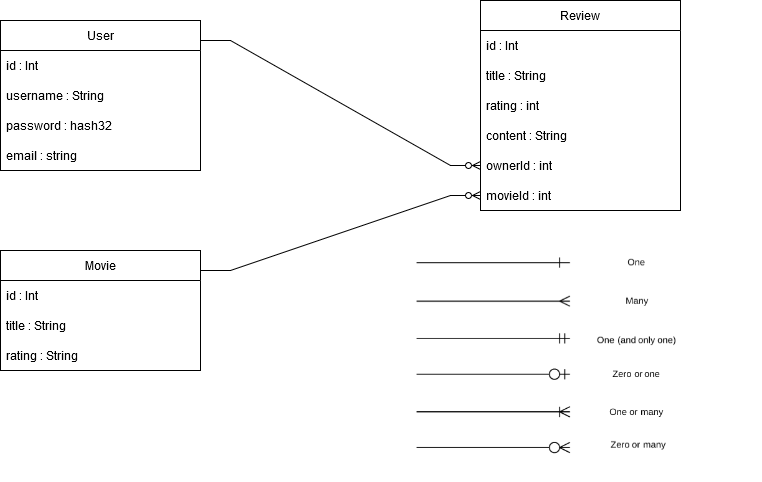
\includegraphics[width=0.8\textwidth]{example-er.png}

    \caption{Modelo Relacional UML da aplicação MyRottenPotatoes.}

    \label{fig:uml}

\end{figure}
 
\section*{Considerações Finais}

O modelo apresentado reflete a simplicidade e eficácia do design da aplicação \textbf{MyRottenPotatoes}, permitindo escalabilidade e fácil manutenção. Ele pode ser expandido para incluir novas funcionalidades, como categorias de filmes ou usuários registrados.
 
\end{document}

 